\documentclass[twoside]{book}

% Packages required by doxygen
\usepackage{calc}
\usepackage{doxygen}
\usepackage{graphicx}
\usepackage[utf8]{inputenc}
\usepackage{makeidx}
\usepackage{multicol}
\usepackage{multirow}
\usepackage{textcomp}
\usepackage[table]{xcolor}

% Font selection
\usepackage[T1]{fontenc}
\usepackage{mathptmx}
\usepackage[scaled=.90]{helvet}
\usepackage{courier}
\usepackage{amssymb}
\usepackage{sectsty}
\renewcommand{\familydefault}{\sfdefault}
\allsectionsfont{%
  \fontseries{bc}\selectfont%
  \color{darkgray}%
}
\renewcommand{\DoxyLabelFont}{%
  \fontseries{bc}\selectfont%
  \color{darkgray}%
}

% Page & text layout
\usepackage{geometry}
\geometry{%
  a4paper,%
  top=2.5cm,%
  bottom=2.5cm,%
  left=2.5cm,%
  right=2.5cm%
}
\tolerance=750
\hfuzz=15pt
\hbadness=750
\setlength{\emergencystretch}{15pt}
\setlength{\parindent}{0cm}
\setlength{\parskip}{0.2cm}
\makeatletter
\renewcommand{\paragraph}{%
  \@startsection{paragraph}{4}{0ex}{-1.0ex}{1.0ex}{%
    \normalfont\normalsize\bfseries\SS@parafont%
  }%
}
\renewcommand{\subparagraph}{%
  \@startsection{subparagraph}{5}{0ex}{-1.0ex}{1.0ex}{%
    \normalfont\normalsize\bfseries\SS@subparafont%
  }%
}
\makeatother

% Headers & footers
\usepackage{fancyhdr}
\pagestyle{fancyplain}
\fancyhead[LE]{\fancyplain{}{\bfseries\thepage}}
\fancyhead[CE]{\fancyplain{}{}}
\fancyhead[RE]{\fancyplain{}{\bfseries\leftmark}}
\fancyhead[LO]{\fancyplain{}{\bfseries\rightmark}}
\fancyhead[CO]{\fancyplain{}{}}
\fancyhead[RO]{\fancyplain{}{\bfseries\thepage}}
\fancyfoot[LE]{\fancyplain{}{}}
\fancyfoot[CE]{\fancyplain{}{}}
\fancyfoot[RE]{\fancyplain{}{\bfseries\scriptsize Generated on Wed Nov 28 2018 16\-:09\-:33 for print\-\_\-ip by Doxygen }}
\fancyfoot[LO]{\fancyplain{}{\bfseries\scriptsize Generated on Wed Nov 28 2018 16\-:09\-:33 for print\-\_\-ip by Doxygen }}
\fancyfoot[CO]{\fancyplain{}{}}
\fancyfoot[RO]{\fancyplain{}{}}
\renewcommand{\footrulewidth}{0.4pt}
\renewcommand{\chaptermark}[1]{%
  \markboth{#1}{}%
}
\renewcommand{\sectionmark}[1]{%
  \markright{\thesection\ #1}%
}

% Indices & bibliography
\usepackage{natbib}
\usepackage[titles]{tocloft}
\setcounter{tocdepth}{3}
\setcounter{secnumdepth}{5}
\makeindex

% Hyperlinks (required, but should be loaded last)
\usepackage{ifpdf}
\ifpdf
  \usepackage[pdftex,pagebackref=true]{hyperref}
\else
  \usepackage[ps2pdf,pagebackref=true]{hyperref}
\fi
\hypersetup{%
  colorlinks=true,%
  linkcolor=blue,%
  citecolor=blue,%
  unicode%
}

% Custom commands
\newcommand{\clearemptydoublepage}{%
  \newpage{\pagestyle{empty}\cleardoublepage}%
}


%===== C O N T E N T S =====

\begin{document}

% Titlepage & ToC
\hypersetup{pageanchor=false}
\pagenumbering{roman}
\begin{titlepage}
\vspace*{7cm}
\begin{center}%
{\Large print\-\_\-ip }\\
\vspace*{1cm}
{\large Generated by Doxygen 1.8.6}\\
\vspace*{0.5cm}
{\small Wed Nov 28 2018 16:09:33}\\
\end{center}
\end{titlepage}
\clearemptydoublepage
\tableofcontents
\clearemptydoublepage
\pagenumbering{arabic}
\hypersetup{pageanchor=true}

%--- Begin generated contents ---
\chapter{Hierarchical Index}
\section{Class Hierarchy}
This inheritance list is sorted roughly, but not completely, alphabetically\-:\begin{DoxyCompactList}
\item \contentsline{section}{cout\-\_\-redirect}{\pageref{structcout__redirect}}{}
\item false\-\_\-type\begin{DoxyCompactList}
\item \contentsline{section}{is\-\_\-container$<$ T $>$}{\pageref{structis__container}}{}
\item \contentsline{section}{is\-\_\-same\-\_\-t$<$ T, U, Args...$>$}{\pageref{structis__same__t_3_01T_00_01U_00_01Args_8_8_8_4}}{}
\end{DoxyCompactList}
\item \contentsline{section}{is\-\_\-same\-\_\-t$<$ T, Args $>$}{\pageref{structis__same__t}}{}
\item \contentsline{section}{is\-\_\-same\-\_\-t$<$ T, Args...$>$}{\pageref{structis__same__t}}{}
\begin{DoxyCompactList}
\item \contentsline{section}{is\-\_\-same\-\_\-t$<$ T, T, Args...$>$}{\pageref{structis__same__t_3_01T_00_01T_00_01Args_8_8_8_4}}{}
\end{DoxyCompactList}
\item true\-\_\-type\begin{DoxyCompactList}
\item \contentsline{section}{is\-\_\-container$<$ std\-:\-:list$<$ T...$>$ $>$}{\pageref{structis__container_3_01std_1_1list_3_01T_8_8_8_4_01_4}}{}
\item \contentsline{section}{is\-\_\-container$<$ std\-:\-:vector$<$ T...$>$ $>$}{\pageref{structis__container_3_01std_1_1vector_3_01T_8_8_8_4_01_4}}{}
\item \contentsline{section}{is\-\_\-same\-\_\-t$<$ T $>$}{\pageref{structis__same__t_3_01T_01_4}}{}
\end{DoxyCompactList}
\item \contentsline{section}{Tuple\-Printer$<$ Tuple, N $>$}{\pageref{structTuplePrinter}}{}
\item \contentsline{section}{Tuple\-Printer$<$ Tuple, 1 $>$}{\pageref{structTuplePrinter_3_01Tuple_00_011_01_4}}{}
\end{DoxyCompactList}

\chapter{Class Index}
\section{Class List}
Here are the classes, structs, unions and interfaces with brief descriptions\-:\begin{DoxyCompactList}
\item\contentsline{section}{\hyperlink{structcout__redirect}{cout\-\_\-redirect} }{\pageref{structcout__redirect}}{}
\item\contentsline{section}{\hyperlink{structis__container}{is\-\_\-container$<$ T $>$} \\*Проверка типа -\/ контейнер }{\pageref{structis__container}}{}
\item\contentsline{section}{\hyperlink{structis__container_3_01std_1_1list_3_01T_8_8_8_4_01_4}{is\-\_\-container$<$ std\-::list$<$ T...$>$ $>$} \\*Проверка типа -\/ контейнер }{\pageref{structis__container_3_01std_1_1list_3_01T_8_8_8_4_01_4}}{}
\item\contentsline{section}{\hyperlink{structis__container_3_01std_1_1vector_3_01T_8_8_8_4_01_4}{is\-\_\-container$<$ std\-::vector$<$ T...$>$ $>$} \\*Проверка типа -\/ контейнер }{\pageref{structis__container_3_01std_1_1vector_3_01T_8_8_8_4_01_4}}{}
\item\contentsline{section}{\hyperlink{structis__same__t}{is\-\_\-same\-\_\-t$<$ T, Args $>$} \\*Проверка на идентичность типов }{\pageref{structis__same__t}}{}
\item\contentsline{section}{\hyperlink{structis__same__t_3_01T_01_4}{is\-\_\-same\-\_\-t$<$ T $>$} \\*Проверка на идентичность типов }{\pageref{structis__same__t_3_01T_01_4}}{}
\item\contentsline{section}{\hyperlink{structis__same__t_3_01T_00_01T_00_01Args_8_8_8_4}{is\-\_\-same\-\_\-t$<$ T, T, Args...$>$} \\*Проверка на идентичность типов }{\pageref{structis__same__t_3_01T_00_01T_00_01Args_8_8_8_4}}{}
\item\contentsline{section}{\hyperlink{structis__same__t_3_01T_00_01U_00_01Args_8_8_8_4}{is\-\_\-same\-\_\-t$<$ T, U, Args...$>$} \\*Проверка на идентичность типов }{\pageref{structis__same__t_3_01T_00_01U_00_01Args_8_8_8_4}}{}
\item\contentsline{section}{\hyperlink{structTuplePrinter}{Tuple\-Printer$<$ Tuple, N $>$} \\*Структура -\/ хелпер для печати кортежа произвольной длины }{\pageref{structTuplePrinter}}{}
\item\contentsline{section}{\hyperlink{structTuplePrinter_3_01Tuple_00_011_01_4}{Tuple\-Printer$<$ Tuple, 1 $>$} \\*Структура -\/ хелпер для печати кортежа произвольной длины }{\pageref{structTuplePrinter_3_01Tuple_00_011_01_4}}{}
\end{DoxyCompactList}

\chapter{File Index}
\section{File List}
Here is a list of all files with brief descriptions\-:\begin{DoxyCompactList}
\item\contentsline{section}{\hyperlink{lib_8cpp}{lib.\-cpp} }{\pageref{lib_8cpp}}{}
\item\contentsline{section}{\hyperlink{lib_8h}{lib.\-h} }{\pageref{lib_8h}}{}
\item\contentsline{section}{\hyperlink{main_8cpp}{main.\-cpp} }{\pageref{main_8cpp}}{}
\item\contentsline{section}{\hyperlink{main__test_8cpp}{main\-\_\-test.\-cpp} }{\pageref{main__test_8cpp}}{}
\item\contentsline{section}{\hyperlink{version_8h}{version.\-h} }{\pageref{version_8h}}{}
\end{DoxyCompactList}

\chapter{Class Documentation}
\hypertarget{structcout__redirect}{\section{cout\-\_\-redirect Struct Reference}
\label{structcout__redirect}\index{cout\-\_\-redirect@{cout\-\_\-redirect}}
}
\subsection*{Public Member Functions}
\begin{DoxyCompactItemize}
\item 
\hyperlink{structcout__redirect_a1ce2b56b3bf54f8bbd2709828e517946}{cout\-\_\-redirect} (std\-::streambuf $\ast$new\-\_\-buffer)
\item 
\hyperlink{structcout__redirect_a6f5fcbfd32ccdc91684fb4c91d170001}{$\sim$cout\-\_\-redirect} ()
\end{DoxyCompactItemize}


\subsection{Constructor \& Destructor Documentation}
\hypertarget{structcout__redirect_a1ce2b56b3bf54f8bbd2709828e517946}{\index{cout\-\_\-redirect@{cout\-\_\-redirect}!cout\-\_\-redirect@{cout\-\_\-redirect}}
\index{cout\-\_\-redirect@{cout\-\_\-redirect}!cout_redirect@{cout\-\_\-redirect}}
\subsubsection[{cout\-\_\-redirect}]{\setlength{\rightskip}{0pt plus 5cm}cout\-\_\-redirect\-::cout\-\_\-redirect (
\begin{DoxyParamCaption}
\item[{std\-::streambuf $\ast$}]{new\-\_\-buffer}
\end{DoxyParamCaption}
)\hspace{0.3cm}{\ttfamily [inline]}}}\label{structcout__redirect_a1ce2b56b3bf54f8bbd2709828e517946}
\hypertarget{structcout__redirect_a6f5fcbfd32ccdc91684fb4c91d170001}{\index{cout\-\_\-redirect@{cout\-\_\-redirect}!$\sim$cout\-\_\-redirect@{$\sim$cout\-\_\-redirect}}
\index{$\sim$cout\-\_\-redirect@{$\sim$cout\-\_\-redirect}!cout_redirect@{cout\-\_\-redirect}}
\subsubsection[{$\sim$cout\-\_\-redirect}]{\setlength{\rightskip}{0pt plus 5cm}cout\-\_\-redirect\-::$\sim$cout\-\_\-redirect (
\begin{DoxyParamCaption}
{}
\end{DoxyParamCaption}
)\hspace{0.3cm}{\ttfamily [inline]}}}\label{structcout__redirect_a6f5fcbfd32ccdc91684fb4c91d170001}


The documentation for this struct was generated from the following file\-:\begin{DoxyCompactItemize}
\item 
\hyperlink{main__test_8cpp}{main\-\_\-test.\-cpp}\end{DoxyCompactItemize}

\hypertarget{structis__container}{\section{is\-\_\-container$<$ T $>$ Struct Template Reference}
\label{structis__container}\index{is\-\_\-container$<$ T $>$@{is\-\_\-container$<$ T $>$}}
}


{\ttfamily \#include $<$lib.\-h$>$}



Inheritance diagram for is\-\_\-container$<$ T $>$\-:
\nopagebreak
\begin{figure}[H]
\begin{center}
\leavevmode
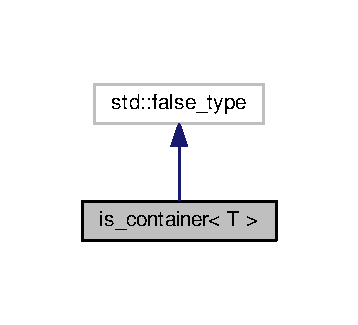
\includegraphics[width=172pt]{structis__container__inherit__graph}
\end{center}
\end{figure}


Collaboration diagram for is\-\_\-container$<$ T $>$\-:
\nopagebreak
\begin{figure}[H]
\begin{center}
\leavevmode
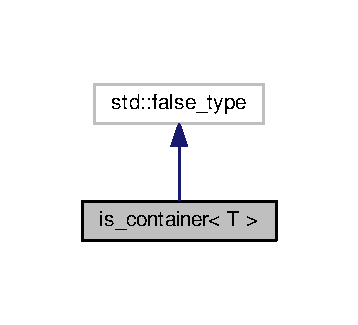
\includegraphics[width=172pt]{structis__container__coll__graph}
\end{center}
\end{figure}


The documentation for this struct was generated from the following file\-:\begin{DoxyCompactItemize}
\item 
\hyperlink{lib_8h}{lib.\-h}\end{DoxyCompactItemize}

\hypertarget{structis__container_3_01std_1_1list_3_01T_8_8_8_4_01_4}{\section{is\-\_\-container$<$ std\-:\-:list$<$ T...$>$ $>$ Struct Template Reference}
\label{structis__container_3_01std_1_1list_3_01T_8_8_8_4_01_4}\index{is\-\_\-container$<$ std\-::list$<$ T...$>$ $>$@{is\-\_\-container$<$ std\-::list$<$ T...$>$ $>$}}
}


Проверка типа -\/ контейнер.  




{\ttfamily \#include $<$lib.\-h$>$}



Inheritance diagram for is\-\_\-container$<$ std\-:\-:list$<$ T...$>$ $>$\-:
\nopagebreak
\begin{figure}[H]
\begin{center}
\leavevmode
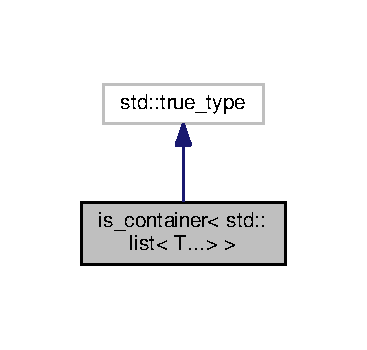
\includegraphics[width=176pt]{structis__container_3_01std_1_1list_3_01T_8_8_8_4_01_4__inherit__graph}
\end{center}
\end{figure}


Collaboration diagram for is\-\_\-container$<$ std\-:\-:list$<$ T...$>$ $>$\-:
\nopagebreak
\begin{figure}[H]
\begin{center}
\leavevmode
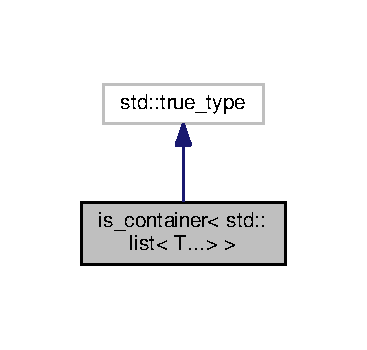
\includegraphics[width=176pt]{structis__container_3_01std_1_1list_3_01T_8_8_8_4_01_4__coll__graph}
\end{center}
\end{figure}


\subsection{Detailed Description}
\subsubsection*{template$<$typename... T$>$struct is\-\_\-container$<$ std\-::list$<$ T...$>$ $>$}

Проверка типа -\/ контейнер. 


\begin{DoxyTemplParams}{Template Parameters}
{\em T} & -\/ тип. \\
\hline
\end{DoxyTemplParams}


The documentation for this struct was generated from the following file\-:\begin{DoxyCompactItemize}
\item 
\hyperlink{lib_8h}{lib.\-h}\end{DoxyCompactItemize}

\hypertarget{structis__container_3_01std_1_1vector_3_01T_8_8_8_4_01_4}{\section{is\-\_\-container$<$ std\-:\-:vector$<$ T...$>$ $>$ Struct Template Reference}
\label{structis__container_3_01std_1_1vector_3_01T_8_8_8_4_01_4}\index{is\-\_\-container$<$ std\-::vector$<$ T...$>$ $>$@{is\-\_\-container$<$ std\-::vector$<$ T...$>$ $>$}}
}


Проверка типа -\/ контейнер.  




{\ttfamily \#include $<$lib.\-h$>$}



Inheritance diagram for is\-\_\-container$<$ std\-:\-:vector$<$ T...$>$ $>$\-:
\nopagebreak
\begin{figure}[H]
\begin{center}
\leavevmode
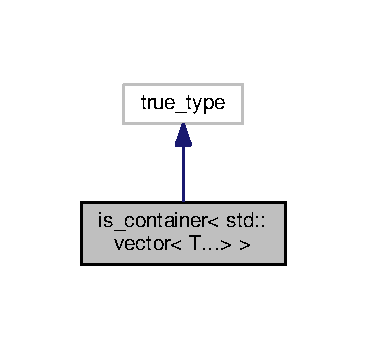
\includegraphics[width=176pt]{structis__container_3_01std_1_1vector_3_01T_8_8_8_4_01_4__inherit__graph}
\end{center}
\end{figure}


Collaboration diagram for is\-\_\-container$<$ std\-:\-:vector$<$ T...$>$ $>$\-:
\nopagebreak
\begin{figure}[H]
\begin{center}
\leavevmode
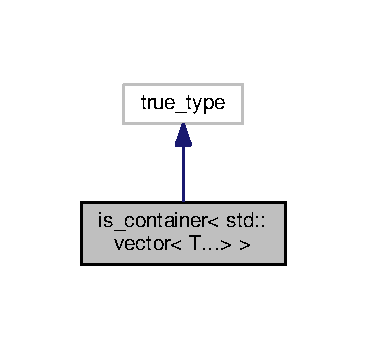
\includegraphics[width=176pt]{structis__container_3_01std_1_1vector_3_01T_8_8_8_4_01_4__coll__graph}
\end{center}
\end{figure}


\subsection{Detailed Description}
\subsubsection*{template$<$typename... T$>$struct is\-\_\-container$<$ std\-::vector$<$ T...$>$ $>$}

Проверка типа -\/ контейнер. 


\begin{DoxyTemplParams}{Template Parameters}
{\em T} & -\/ тип. \\
\hline
\end{DoxyTemplParams}


The documentation for this struct was generated from the following file\-:\begin{DoxyCompactItemize}
\item 
\hyperlink{lib_8h}{lib.\-h}\end{DoxyCompactItemize}

\hypertarget{structis__same__t}{\section{is\-\_\-same\-\_\-t$<$ T, Args $>$ Struct Template Reference}
\label{structis__same__t}\index{is\-\_\-same\-\_\-t$<$ T, Args $>$@{is\-\_\-same\-\_\-t$<$ T, Args $>$}}
}


{\ttfamily \#include $<$lib.\-h$>$}



The documentation for this struct was generated from the following file\-:\begin{DoxyCompactItemize}
\item 
\hyperlink{lib_8h}{lib.\-h}\end{DoxyCompactItemize}

\hypertarget{structis__same__t_3_01T_01_4}{\section{is\-\_\-same\-\_\-t$<$ T $>$ Struct Template Reference}
\label{structis__same__t_3_01T_01_4}\index{is\-\_\-same\-\_\-t$<$ T $>$@{is\-\_\-same\-\_\-t$<$ T $>$}}
}


Проверка на идентичность типов.  




{\ttfamily \#include $<$lib.\-h$>$}



Inheritance diagram for is\-\_\-same\-\_\-t$<$ T $>$\-:
\nopagebreak
\begin{figure}[H]
\begin{center}
\leavevmode
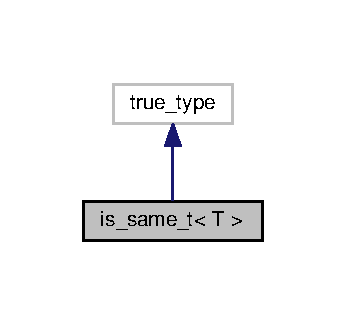
\includegraphics[width=166pt]{structis__same__t_3_01T_01_4__inherit__graph}
\end{center}
\end{figure}


Collaboration diagram for is\-\_\-same\-\_\-t$<$ T $>$\-:
\nopagebreak
\begin{figure}[H]
\begin{center}
\leavevmode
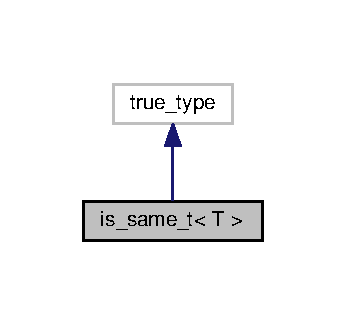
\includegraphics[width=166pt]{structis__same__t_3_01T_01_4__coll__graph}
\end{center}
\end{figure}


\subsection{Detailed Description}
\subsubsection*{template$<$typename T$>$struct is\-\_\-same\-\_\-t$<$ T $>$}

Проверка на идентичность типов. 

The documentation for this struct was generated from the following file\-:\begin{DoxyCompactItemize}
\item 
\hyperlink{lib_8h}{lib.\-h}\end{DoxyCompactItemize}

\hypertarget{structis__same__t_3_01T_00_01T_00_01Args_8_8_8_4}{\section{is\-\_\-same\-\_\-t$<$ T, T, Args...$>$ Struct Template Reference}
\label{structis__same__t_3_01T_00_01T_00_01Args_8_8_8_4}\index{is\-\_\-same\-\_\-t$<$ T, T, Args...$>$@{is\-\_\-same\-\_\-t$<$ T, T, Args...$>$}}
}


Проверка на идентичность типов.  




{\ttfamily \#include $<$lib.\-h$>$}



Inheritance diagram for is\-\_\-same\-\_\-t$<$ T, T, Args...$>$\-:
\nopagebreak
\begin{figure}[H]
\begin{center}
\leavevmode
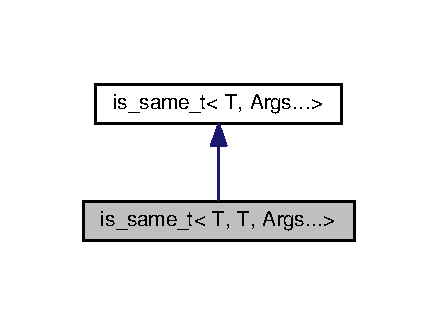
\includegraphics[width=210pt]{structis__same__t_3_01T_00_01T_00_01Args_8_8_8_4__inherit__graph}
\end{center}
\end{figure}


Collaboration diagram for is\-\_\-same\-\_\-t$<$ T, T, Args...$>$\-:
\nopagebreak
\begin{figure}[H]
\begin{center}
\leavevmode
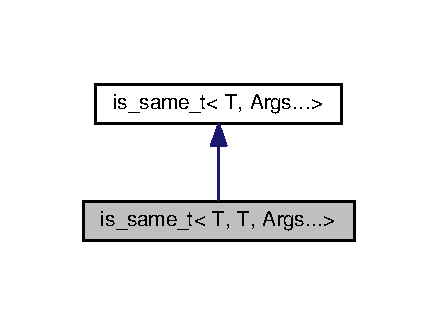
\includegraphics[width=210pt]{structis__same__t_3_01T_00_01T_00_01Args_8_8_8_4__coll__graph}
\end{center}
\end{figure}


\subsection{Detailed Description}
\subsubsection*{template$<$typename T, typename... Args$>$struct is\-\_\-same\-\_\-t$<$ T, T, Args...$>$}

Проверка на идентичность типов. 

The documentation for this struct was generated from the following file\-:\begin{DoxyCompactItemize}
\item 
\hyperlink{lib_8h}{lib.\-h}\end{DoxyCompactItemize}

\hypertarget{structis__same__t_3_01T_00_01U_00_01Args_8_8_8_4}{\section{is\-\_\-same\-\_\-t$<$ T, U, Args...$>$ Struct Template Reference}
\label{structis__same__t_3_01T_00_01U_00_01Args_8_8_8_4}\index{is\-\_\-same\-\_\-t$<$ T, U, Args...$>$@{is\-\_\-same\-\_\-t$<$ T, U, Args...$>$}}
}


{\ttfamily \#include $<$lib.\-h$>$}



Inheritance diagram for is\-\_\-same\-\_\-t$<$ T, U, Args...$>$\-:
\nopagebreak
\begin{figure}[H]
\begin{center}
\leavevmode
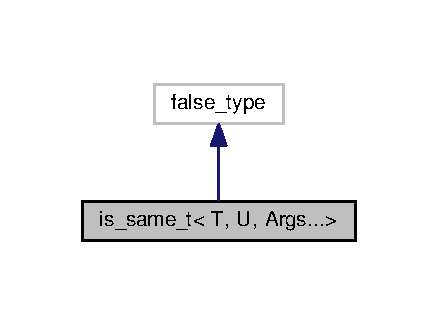
\includegraphics[width=210pt]{structis__same__t_3_01T_00_01U_00_01Args_8_8_8_4__inherit__graph}
\end{center}
\end{figure}


Collaboration diagram for is\-\_\-same\-\_\-t$<$ T, U, Args...$>$\-:
\nopagebreak
\begin{figure}[H]
\begin{center}
\leavevmode
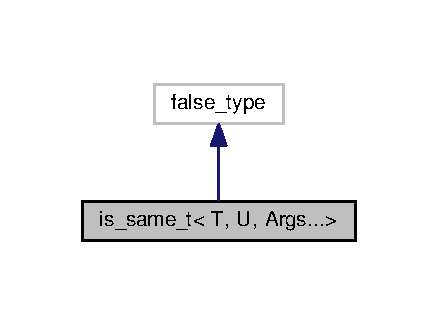
\includegraphics[width=210pt]{structis__same__t_3_01T_00_01U_00_01Args_8_8_8_4__coll__graph}
\end{center}
\end{figure}


The documentation for this struct was generated from the following file\-:\begin{DoxyCompactItemize}
\item 
\hyperlink{lib_8h}{lib.\-h}\end{DoxyCompactItemize}

\hypertarget{structTuplePrinter}{\section{Tuple\-Printer$<$ Tuple, N $>$ Struct Template Reference}
\label{structTuplePrinter}\index{Tuple\-Printer$<$ Tuple, N $>$@{Tuple\-Printer$<$ Tuple, N $>$}}
}


{\ttfamily \#include $<$lib.\-h$>$}

\subsection*{Static Public Member Functions}
\begin{DoxyCompactItemize}
\item 
static void \hyperlink{structTuplePrinter_aaf76573f278205ba63759d5dbe3f408c}{print} (const Tuple \&t)
\end{DoxyCompactItemize}


\subsection{Member Function Documentation}
\hypertarget{structTuplePrinter_aaf76573f278205ba63759d5dbe3f408c}{\index{Tuple\-Printer@{Tuple\-Printer}!print@{print}}
\index{print@{print}!TuplePrinter@{Tuple\-Printer}}
\subsubsection[{print}]{\setlength{\rightskip}{0pt plus 5cm}template$<$class Tuple , size\-\_\-t N$>$ static void {\bf Tuple\-Printer}$<$ Tuple, N $>$\-::print (
\begin{DoxyParamCaption}
\item[{const Tuple \&}]{t}
\end{DoxyParamCaption}
)\hspace{0.3cm}{\ttfamily [inline]}, {\ttfamily [static]}}}\label{structTuplePrinter_aaf76573f278205ba63759d5dbe3f408c}


The documentation for this struct was generated from the following file\-:\begin{DoxyCompactItemize}
\item 
\hyperlink{lib_8h}{lib.\-h}\end{DoxyCompactItemize}

\hypertarget{structTuplePrinter_3_01Tuple_00_011_01_4}{\section{Tuple\-Printer$<$ Tuple, 1 $>$ Struct Template Reference}
\label{structTuplePrinter_3_01Tuple_00_011_01_4}\index{Tuple\-Printer$<$ Tuple, 1 $>$@{Tuple\-Printer$<$ Tuple, 1 $>$}}
}


{\ttfamily \#include $<$lib.\-h$>$}

\subsection*{Static Public Member Functions}
\begin{DoxyCompactItemize}
\item 
static void \hyperlink{structTuplePrinter_3_01Tuple_00_011_01_4_af4ab0b518a1d2927e949c817aa6b7266}{print} (const Tuple \&t)
\end{DoxyCompactItemize}


\subsection{Member Function Documentation}
\hypertarget{structTuplePrinter_3_01Tuple_00_011_01_4_af4ab0b518a1d2927e949c817aa6b7266}{\index{Tuple\-Printer$<$ Tuple, 1 $>$@{Tuple\-Printer$<$ Tuple, 1 $>$}!print@{print}}
\index{print@{print}!TuplePrinter< Tuple, 1 >@{Tuple\-Printer$<$ Tuple, 1 $>$}}
\subsubsection[{print}]{\setlength{\rightskip}{0pt plus 5cm}template$<$class Tuple $>$ static void {\bf Tuple\-Printer}$<$ Tuple, 1 $>$\-::print (
\begin{DoxyParamCaption}
\item[{const Tuple \&}]{t}
\end{DoxyParamCaption}
)\hspace{0.3cm}{\ttfamily [inline]}, {\ttfamily [static]}}}\label{structTuplePrinter_3_01Tuple_00_011_01_4_af4ab0b518a1d2927e949c817aa6b7266}


The documentation for this struct was generated from the following file\-:\begin{DoxyCompactItemize}
\item 
\hyperlink{lib_8h}{lib.\-h}\end{DoxyCompactItemize}

\chapter{File Documentation}
\hypertarget{lib_8cpp}{\section{lib.\-cpp File Reference}
\label{lib_8cpp}\index{lib.\-cpp@{lib.\-cpp}}
}
{\ttfamily \#include \char`\"{}lib.\-h\char`\"{}}\\*
Include dependency graph for lib.\-cpp\-:
\nopagebreak
\begin{figure}[H]
\begin{center}
\leavevmode
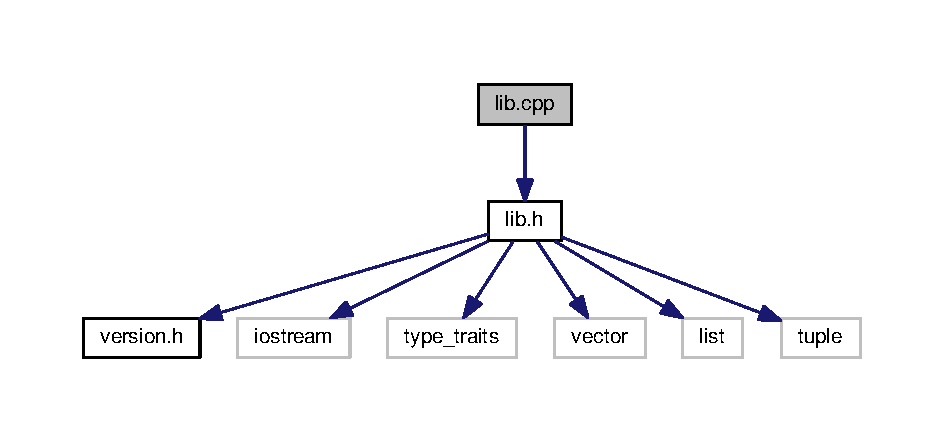
\includegraphics[width=350pt]{lib_8cpp__incl}
\end{center}
\end{figure}
\subsection*{Functions}
\begin{DoxyCompactItemize}
\item 
int \hyperlink{lib_8cpp_ae64f17a84dc9c7144d1036498ff26fd9}{version} ()
\begin{DoxyCompactList}\small\item\em version Получение версии. \end{DoxyCompactList}\end{DoxyCompactItemize}


\subsection{Function Documentation}
\hypertarget{lib_8cpp_ae64f17a84dc9c7144d1036498ff26fd9}{\index{lib.\-cpp@{lib.\-cpp}!version@{version}}
\index{version@{version}!lib.cpp@{lib.\-cpp}}
\subsubsection[{version}]{\setlength{\rightskip}{0pt plus 5cm}int version (
\begin{DoxyParamCaption}
{}
\end{DoxyParamCaption}
)}}\label{lib_8cpp_ae64f17a84dc9c7144d1036498ff26fd9}


version Получение версии. 

\begin{DoxyReturn}{Returns}
Номер версии. 
\end{DoxyReturn}

\hypertarget{lib_8h}{\section{lib.\-h File Reference}
\label{lib_8h}\index{lib.\-h@{lib.\-h}}
}
{\ttfamily \#include \char`\"{}version.\-h\char`\"{}}\\*
{\ttfamily \#include $<$iostream$>$}\\*
{\ttfamily \#include $<$type\-\_\-traits$>$}\\*
{\ttfamily \#include $<$vector$>$}\\*
{\ttfamily \#include $<$list$>$}\\*
{\ttfamily \#include $<$tuple$>$}\\*
Include dependency graph for lib.\-h\-:
\nopagebreak
\begin{figure}[H]
\begin{center}
\leavevmode
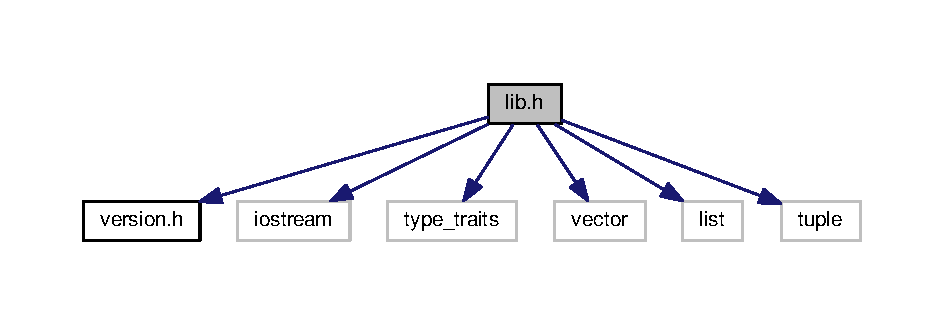
\includegraphics[width=350pt]{lib_8h__incl}
\end{center}
\end{figure}
This graph shows which files directly or indirectly include this file\-:
\nopagebreak
\begin{figure}[H]
\begin{center}
\leavevmode
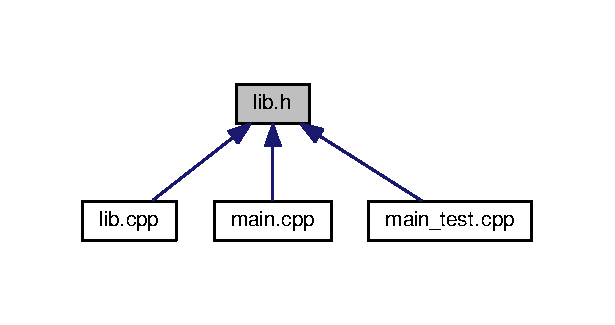
\includegraphics[width=295pt]{lib_8h__dep__incl}
\end{center}
\end{figure}
\subsection*{Classes}
\begin{DoxyCompactItemize}
\item 
struct \hyperlink{structis__container}{is\-\_\-container$<$ T $>$}
\begin{DoxyCompactList}\small\item\em Проверка типа -\/ контейнер. \end{DoxyCompactList}\item 
struct \hyperlink{structis__container_3_01std_1_1vector_3_01T_8_8_8_4_01_4}{is\-\_\-container$<$ std\-::vector$<$ T...$>$ $>$}
\begin{DoxyCompactList}\small\item\em Проверка типа -\/ контейнер. \end{DoxyCompactList}\item 
struct \hyperlink{structis__container_3_01std_1_1list_3_01T_8_8_8_4_01_4}{is\-\_\-container$<$ std\-::list$<$ T...$>$ $>$}
\begin{DoxyCompactList}\small\item\em Проверка типа -\/ контейнер. \end{DoxyCompactList}\item 
struct \hyperlink{structis__same__t}{is\-\_\-same\-\_\-t$<$ T, Args $>$}
\begin{DoxyCompactList}\small\item\em Проверка на идентичность типов. \end{DoxyCompactList}\item 
struct \hyperlink{structis__same__t_3_01T_01_4}{is\-\_\-same\-\_\-t$<$ T $>$}
\begin{DoxyCompactList}\small\item\em Проверка на идентичность типов. \end{DoxyCompactList}\item 
struct \hyperlink{structis__same__t_3_01T_00_01U_00_01Args_8_8_8_4}{is\-\_\-same\-\_\-t$<$ T, U, Args...$>$}
\begin{DoxyCompactList}\small\item\em Проверка на идентичность типов. \end{DoxyCompactList}\item 
struct \hyperlink{structis__same__t_3_01T_00_01T_00_01Args_8_8_8_4}{is\-\_\-same\-\_\-t$<$ T, T, Args...$>$}
\begin{DoxyCompactList}\small\item\em Проверка на идентичность типов. \end{DoxyCompactList}\item 
struct \hyperlink{structTuplePrinter}{Tuple\-Printer$<$ Tuple, N $>$}
\begin{DoxyCompactList}\small\item\em Структура -\/ хелпер для печати кортежа произвольной длины. \end{DoxyCompactList}\item 
struct \hyperlink{structTuplePrinter_3_01Tuple_00_011_01_4}{Tuple\-Printer$<$ Tuple, 1 $>$}
\begin{DoxyCompactList}\small\item\em Структура -\/ хелпер для печати кортежа произвольной длины. \end{DoxyCompactList}\end{DoxyCompactItemize}
\subsection*{Functions}
\begin{DoxyCompactItemize}
\item 
int \hyperlink{lib_8h_ae64f17a84dc9c7144d1036498ff26fd9}{version} ()
\begin{DoxyCompactList}\small\item\em version Получение версии. \end{DoxyCompactList}\item 
{\footnotesize template$<$typename T $>$ }\\unsigned char \hyperlink{lib_8h_adcf537f99d43dc6d746c61025eef962d}{integral\-Byte} (const T \&val, const char \&n)
\begin{DoxyCompactList}\small\item\em Получение конкретного байта числа. \end{DoxyCompactList}\item 
{\footnotesize template$<$typename T $>$ }\\std\-::enable\-\_\-if\-\_\-t\\*
$<$ std\-::is\-\_\-integral$<$ T $>$\-::value $>$ \hyperlink{lib_8h_a6ed74af6a137d944e7c6d7aa831fde15}{print\-\_\-ip} (const T \&val)
\begin{DoxyCompactList}\small\item\em Печать ip-\/адреса в интегральном виде. \end{DoxyCompactList}\item 
void \hyperlink{lib_8h_a0992bea83d590061735494a2ed7fd653}{print\-\_\-ip} (const std\-::string \&val)
\begin{DoxyCompactList}\small\item\em Печать ip-\/адреса в строковом виде. \end{DoxyCompactList}\item 
{\footnotesize template$<$typename T $>$ }\\std\-::enable\-\_\-if\-\_\-t$<$ \hyperlink{structis__container}{is\-\_\-container}\\*
$<$ T $>$\-::value $>$ \hyperlink{lib_8h_af620902388f12a15b227bc860fc02a26}{print\-\_\-ip} (const T \&val)
\begin{DoxyCompactList}\small\item\em Печать ip-\/адреса в виде контейнера. \end{DoxyCompactList}\item 
{\footnotesize template$<$typename... Args$>$ }\\std\-::enable\-\_\-if$<$ \hyperlink{structis__same__t}{is\-\_\-same\-\_\-t}\\*
$<$ Args...$>$\-::value $>$\-::type \hyperlink{lib_8h_a1f7c08e0d4b6ed4afe8bff90f21fe16c}{print\-\_\-ip} (const std\-::tuple$<$ Args...$>$ \&val)
\begin{DoxyCompactList}\small\item\em Печать ip-\/адреса в виде кортежа. \end{DoxyCompactList}\end{DoxyCompactItemize}


\subsection{Function Documentation}
\hypertarget{lib_8h_adcf537f99d43dc6d746c61025eef962d}{\index{lib.\-h@{lib.\-h}!integral\-Byte@{integral\-Byte}}
\index{integral\-Byte@{integral\-Byte}!lib.h@{lib.\-h}}
\subsubsection[{integral\-Byte}]{\setlength{\rightskip}{0pt plus 5cm}template$<$typename T $>$ unsigned char integral\-Byte (
\begin{DoxyParamCaption}
\item[{const T \&}]{val, }
\item[{const char \&}]{n}
\end{DoxyParamCaption}
)}}\label{lib_8h_adcf537f99d43dc6d746c61025eef962d}


Получение конкретного байта числа. 


\begin{DoxyTemplParams}{Template Parameters}
{\em T} & -\/ интегральный тип. \\
\hline
\end{DoxyTemplParams}

\begin{DoxyParams}{Parameters}
{\em val} & -\/ число. \\
\hline
{\em n} & -\/ номер байта. \\
\hline
\end{DoxyParams}
\begin{DoxyReturn}{Returns}
Искомый байт. 
\end{DoxyReturn}
\hypertarget{lib_8h_a6ed74af6a137d944e7c6d7aa831fde15}{\index{lib.\-h@{lib.\-h}!print\-\_\-ip@{print\-\_\-ip}}
\index{print\-\_\-ip@{print\-\_\-ip}!lib.h@{lib.\-h}}
\subsubsection[{print\-\_\-ip}]{\setlength{\rightskip}{0pt plus 5cm}template$<$typename T $>$ std\-::enable\-\_\-if\-\_\-t$<$std\-::is\-\_\-integral$<$T$>$\-::value$>$ print\-\_\-ip (
\begin{DoxyParamCaption}
\item[{const T \&}]{val}
\end{DoxyParamCaption}
)}}\label{lib_8h_a6ed74af6a137d944e7c6d7aa831fde15}


Печать ip-\/адреса в интегральном виде. 


\begin{DoxyTemplParams}{Template Parameters}
{\em T} & -\/ интегральный тип. \\
\hline
\end{DoxyTemplParams}

\begin{DoxyParams}{Parameters}
{\em val} & -\/ значение ip-\/адреса. \\
\hline
\end{DoxyParams}
\hypertarget{lib_8h_a0992bea83d590061735494a2ed7fd653}{\index{lib.\-h@{lib.\-h}!print\-\_\-ip@{print\-\_\-ip}}
\index{print\-\_\-ip@{print\-\_\-ip}!lib.h@{lib.\-h}}
\subsubsection[{print\-\_\-ip}]{\setlength{\rightskip}{0pt plus 5cm}void print\-\_\-ip (
\begin{DoxyParamCaption}
\item[{const std\-::string \&}]{val}
\end{DoxyParamCaption}
)}}\label{lib_8h_a0992bea83d590061735494a2ed7fd653}


Печать ip-\/адреса в строковом виде. 


\begin{DoxyParams}{Parameters}
{\em val} & -\/ значение ip-\/адреса. \\
\hline
\end{DoxyParams}
\hypertarget{lib_8h_af620902388f12a15b227bc860fc02a26}{\index{lib.\-h@{lib.\-h}!print\-\_\-ip@{print\-\_\-ip}}
\index{print\-\_\-ip@{print\-\_\-ip}!lib.h@{lib.\-h}}
\subsubsection[{print\-\_\-ip}]{\setlength{\rightskip}{0pt plus 5cm}template$<$typename T $>$ std\-::enable\-\_\-if\-\_\-t$<${\bf is\-\_\-container}$<$T$>$\-::value$>$ print\-\_\-ip (
\begin{DoxyParamCaption}
\item[{const T \&}]{val}
\end{DoxyParamCaption}
)}}\label{lib_8h_af620902388f12a15b227bc860fc02a26}


Печать ip-\/адреса в виде контейнера. 


\begin{DoxyTemplParams}{Template Parameters}
{\em T} & -\/ тип. \\
\hline
\end{DoxyTemplParams}

\begin{DoxyParams}{Parameters}
{\em val} & -\/ значение ip-\/адреса. \\
\hline
\end{DoxyParams}
\hypertarget{lib_8h_a1f7c08e0d4b6ed4afe8bff90f21fe16c}{\index{lib.\-h@{lib.\-h}!print\-\_\-ip@{print\-\_\-ip}}
\index{print\-\_\-ip@{print\-\_\-ip}!lib.h@{lib.\-h}}
\subsubsection[{print\-\_\-ip}]{\setlength{\rightskip}{0pt plus 5cm}template$<$typename... Args$>$ std\-::enable\-\_\-if$<${\bf is\-\_\-same\-\_\-t}$<$Args...$>$\-::value$>$\-::type print\-\_\-ip (
\begin{DoxyParamCaption}
\item[{const std\-::tuple$<$ Args...$>$ \&}]{val}
\end{DoxyParamCaption}
)}}\label{lib_8h_a1f7c08e0d4b6ed4afe8bff90f21fe16c}


Печать ip-\/адреса в виде кортежа. 


\begin{DoxyTemplParams}{Template Parameters}
{\em Args} & -\/ типы членов кортежа. \\
\hline
\end{DoxyTemplParams}

\begin{DoxyParams}{Parameters}
{\em val} & -\/ значение ip-\/адреса. \\
\hline
\end{DoxyParams}
\hypertarget{lib_8h_ae64f17a84dc9c7144d1036498ff26fd9}{\index{lib.\-h@{lib.\-h}!version@{version}}
\index{version@{version}!lib.h@{lib.\-h}}
\subsubsection[{version}]{\setlength{\rightskip}{0pt plus 5cm}int version (
\begin{DoxyParamCaption}
{}
\end{DoxyParamCaption}
)}}\label{lib_8h_ae64f17a84dc9c7144d1036498ff26fd9}


version Получение версии. 

\begin{DoxyReturn}{Returns}
Номер версии. 
\end{DoxyReturn}

\hypertarget{main_8cpp}{\section{main.\-cpp File Reference}
\label{main_8cpp}\index{main.\-cpp@{main.\-cpp}}
}
{\ttfamily \#include \char`\"{}lib.\-h\char`\"{}}\\*
{\ttfamily \#include $<$vector$>$}\\*
{\ttfamily \#include $<$list$>$}\\*
{\ttfamily \#include $<$tuple$>$}\\*
Include dependency graph for main.\-cpp\-:
\nopagebreak
\begin{figure}[H]
\begin{center}
\leavevmode
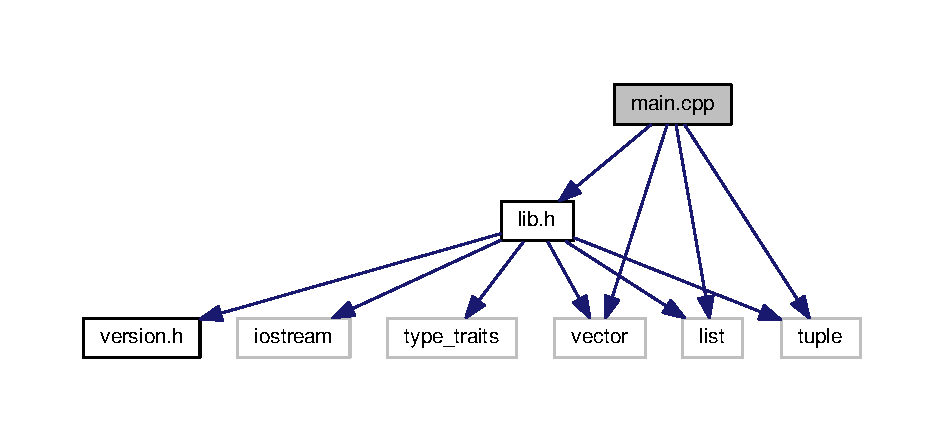
\includegraphics[width=350pt]{main_8cpp__incl}
\end{center}
\end{figure}
\subsection*{Functions}
\begin{DoxyCompactItemize}
\item 
int \hyperlink{main_8cpp_ae66f6b31b5ad750f1fe042a706a4e3d4}{main} ()
\end{DoxyCompactItemize}


\subsection{Function Documentation}
\hypertarget{main_8cpp_ae66f6b31b5ad750f1fe042a706a4e3d4}{\index{main.\-cpp@{main.\-cpp}!main@{main}}
\index{main@{main}!main.cpp@{main.\-cpp}}
\subsubsection[{main}]{\setlength{\rightskip}{0pt plus 5cm}int main (
\begin{DoxyParamCaption}
{}
\end{DoxyParamCaption}
)}}\label{main_8cpp_ae66f6b31b5ad750f1fe042a706a4e3d4}

\hypertarget{main__test_8cpp}{\section{main\-\_\-test.\-cpp File Reference}
\label{main__test_8cpp}\index{main\-\_\-test.\-cpp@{main\-\_\-test.\-cpp}}
}
{\ttfamily \#include \char`\"{}lib.\-h\char`\"{}}\\*
{\ttfamily \#include $<$boost/test/unit\-\_\-test.\-hpp$>$}\\*
{\ttfamily \#include $<$boost/test/output\-\_\-test\-\_\-stream.\-hpp$>$}\\*
Include dependency graph for main\-\_\-test.\-cpp\-:
\nopagebreak
\begin{figure}[H]
\begin{center}
\leavevmode
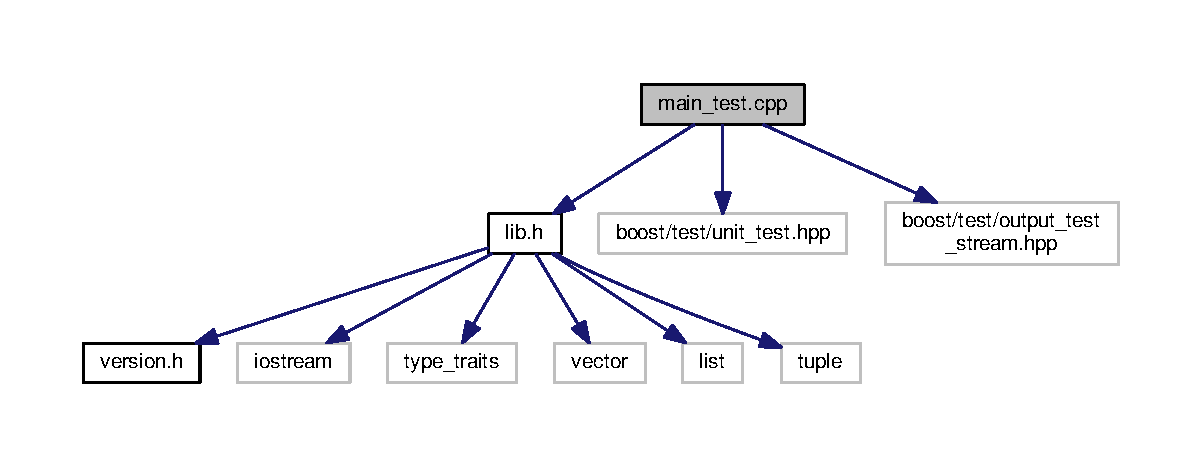
\includegraphics[width=350pt]{main__test_8cpp__incl}
\end{center}
\end{figure}
\subsection*{Classes}
\begin{DoxyCompactItemize}
\item 
struct \hyperlink{structcout__redirect}{cout\-\_\-redirect}
\end{DoxyCompactItemize}
\subsection*{Macros}
\begin{DoxyCompactItemize}
\item 
\#define \hyperlink{main__test_8cpp_a6b2a3852db8bb19ab6909bac01859985}{B\-O\-O\-S\-T\-\_\-\-T\-E\-S\-T\-\_\-\-M\-O\-D\-U\-L\-E}~project\-\_\-test
\end{DoxyCompactItemize}
\subsection*{Typedefs}
\begin{DoxyCompactItemize}
\item 
using \hyperlink{main__test_8cpp_a2fdd3776ac4ce266caa97ebebe59cbe1}{test\-\_\-stream} = boost\-::test\-\_\-tools\-::output\-\_\-test\-\_\-stream
\end{DoxyCompactItemize}
\subsection*{Functions}
\begin{DoxyCompactItemize}
\item 
\hyperlink{main__test_8cpp_a5491eb5660094f9ba5f6a65c5bedffa6}{B\-O\-O\-S\-T\-\_\-\-A\-U\-T\-O\-\_\-\-T\-E\-S\-T\-\_\-\-C\-A\-S\-E} (test\-\_\-print\-\_\-ip)
\end{DoxyCompactItemize}


\subsection{Macro Definition Documentation}
\hypertarget{main__test_8cpp_a6b2a3852db8bb19ab6909bac01859985}{\index{main\-\_\-test.\-cpp@{main\-\_\-test.\-cpp}!B\-O\-O\-S\-T\-\_\-\-T\-E\-S\-T\-\_\-\-M\-O\-D\-U\-L\-E@{B\-O\-O\-S\-T\-\_\-\-T\-E\-S\-T\-\_\-\-M\-O\-D\-U\-L\-E}}
\index{B\-O\-O\-S\-T\-\_\-\-T\-E\-S\-T\-\_\-\-M\-O\-D\-U\-L\-E@{B\-O\-O\-S\-T\-\_\-\-T\-E\-S\-T\-\_\-\-M\-O\-D\-U\-L\-E}!main_test.cpp@{main\-\_\-test.\-cpp}}
\subsubsection[{B\-O\-O\-S\-T\-\_\-\-T\-E\-S\-T\-\_\-\-M\-O\-D\-U\-L\-E}]{\setlength{\rightskip}{0pt plus 5cm}\#define B\-O\-O\-S\-T\-\_\-\-T\-E\-S\-T\-\_\-\-M\-O\-D\-U\-L\-E~project\-\_\-test}}\label{main__test_8cpp_a6b2a3852db8bb19ab6909bac01859985}


\subsection{Typedef Documentation}
\hypertarget{main__test_8cpp_a2fdd3776ac4ce266caa97ebebe59cbe1}{\index{main\-\_\-test.\-cpp@{main\-\_\-test.\-cpp}!test\-\_\-stream@{test\-\_\-stream}}
\index{test\-\_\-stream@{test\-\_\-stream}!main_test.cpp@{main\-\_\-test.\-cpp}}
\subsubsection[{test\-\_\-stream}]{\setlength{\rightskip}{0pt plus 5cm}using {\bf test\-\_\-stream} =  boost\-::test\-\_\-tools\-::output\-\_\-test\-\_\-stream}}\label{main__test_8cpp_a2fdd3776ac4ce266caa97ebebe59cbe1}


\subsection{Function Documentation}
\hypertarget{main__test_8cpp_a5491eb5660094f9ba5f6a65c5bedffa6}{\index{main\-\_\-test.\-cpp@{main\-\_\-test.\-cpp}!B\-O\-O\-S\-T\-\_\-\-A\-U\-T\-O\-\_\-\-T\-E\-S\-T\-\_\-\-C\-A\-S\-E@{B\-O\-O\-S\-T\-\_\-\-A\-U\-T\-O\-\_\-\-T\-E\-S\-T\-\_\-\-C\-A\-S\-E}}
\index{B\-O\-O\-S\-T\-\_\-\-A\-U\-T\-O\-\_\-\-T\-E\-S\-T\-\_\-\-C\-A\-S\-E@{B\-O\-O\-S\-T\-\_\-\-A\-U\-T\-O\-\_\-\-T\-E\-S\-T\-\_\-\-C\-A\-S\-E}!main_test.cpp@{main\-\_\-test.\-cpp}}
\subsubsection[{B\-O\-O\-S\-T\-\_\-\-A\-U\-T\-O\-\_\-\-T\-E\-S\-T\-\_\-\-C\-A\-S\-E}]{\setlength{\rightskip}{0pt plus 5cm}B\-O\-O\-S\-T\-\_\-\-A\-U\-T\-O\-\_\-\-T\-E\-S\-T\-\_\-\-C\-A\-S\-E (
\begin{DoxyParamCaption}
\item[{test\-\_\-print\-\_\-ip}]{}
\end{DoxyParamCaption}
)}}\label{main__test_8cpp_a5491eb5660094f9ba5f6a65c5bedffa6}

\hypertarget{version_8h}{\section{version.\-h File Reference}
\label{version_8h}\index{version.\-h@{version.\-h}}
}
This graph shows which files directly or indirectly include this file\-:
\nopagebreak
\begin{figure}[H]
\begin{center}
\leavevmode
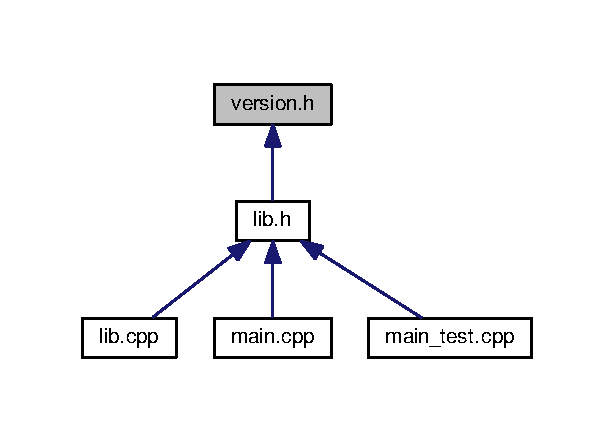
\includegraphics[width=295pt]{version_8h__dep__incl}
\end{center}
\end{figure}
\subsection*{Macros}
\begin{DoxyCompactItemize}
\item 
\#define \hyperlink{version_8h_a4a5fc96a4bdd7d68ed99ccce9ca2e77e}{P\-R\-O\-J\-E\-C\-T\-\_\-\-V\-E\-R\-S\-I\-O\-N\-\_\-\-P\-A\-T\-C\-H}~11
\end{DoxyCompactItemize}


\subsection{Macro Definition Documentation}
\hypertarget{version_8h_a4a5fc96a4bdd7d68ed99ccce9ca2e77e}{\index{version.\-h@{version.\-h}!P\-R\-O\-J\-E\-C\-T\-\_\-\-V\-E\-R\-S\-I\-O\-N\-\_\-\-P\-A\-T\-C\-H@{P\-R\-O\-J\-E\-C\-T\-\_\-\-V\-E\-R\-S\-I\-O\-N\-\_\-\-P\-A\-T\-C\-H}}
\index{P\-R\-O\-J\-E\-C\-T\-\_\-\-V\-E\-R\-S\-I\-O\-N\-\_\-\-P\-A\-T\-C\-H@{P\-R\-O\-J\-E\-C\-T\-\_\-\-V\-E\-R\-S\-I\-O\-N\-\_\-\-P\-A\-T\-C\-H}!version.h@{version.\-h}}
\subsubsection[{P\-R\-O\-J\-E\-C\-T\-\_\-\-V\-E\-R\-S\-I\-O\-N\-\_\-\-P\-A\-T\-C\-H}]{\setlength{\rightskip}{0pt plus 5cm}\#define P\-R\-O\-J\-E\-C\-T\-\_\-\-V\-E\-R\-S\-I\-O\-N\-\_\-\-P\-A\-T\-C\-H~11}}\label{version_8h_a4a5fc96a4bdd7d68ed99ccce9ca2e77e}

%--- End generated contents ---

% Index
\newpage
\phantomsection
\addcontentsline{toc}{chapter}{Index}
\printindex

\end{document}
